\documentclass[10pt,a4paper]{article}
\usepackage[utf8]{inputenc}
\usepackage[italian]{babel}
\usepackage[a4paper]{geometry}
\usepackage{amsmath}
\usepackage{amsthm}
\usepackage{dsfont}
\usepackage{xfrac}
\usepackage{amsfonts}
\usepackage{amssymb}
\usepackage{graphicx}
\usepackage{braket}
\usepackage{mathtools}
\usepackage{booktabs}
\usepackage{hyperref}
\usepackage{enumerate}
\usepackage{pgf,tikz}
\usepackage{mathrsfs}
\usetikzlibrary{arrows}
\DeclarePairedDelimiterX{\norm}[1]{\lVert}{\rVert}{#1}
\theoremstyle{plain}
\newtheorem{definizione}[subsection]{Definizione}
\theoremstyle{definition}
\newtheorem{teorema}[subsection]{Teorema}
\newtheorem{dimostrazione}[subsection]{Dimostrazione}
\newtheorem{corollario}[subsection]{Corollario}
\newtheorem{osservazione}[subsection]{Osservazione}
\newtheorem{proposizione}[subsection]{Proposizione}
\newtheorem{esempio}[subsection]{Esempio}
%%%%%%%INSERIAMO QUI I NUOVI COMANDI %%%%%%%%%%%%%%%%%%%%%%%%%%%%%%%%%%%%%%%%%%%%
\DeclarePairedDelimiterX{\abla}[1]{abla}{abla}{#1}

%%%%%%%QUI VANNO INSERITI IL TITOLO E GLI AUTORI%%%%%%%%%%%%%%%%%%%%%%%%%%%%
\author{Andrea Zanin}
\title{Appunti Matematica Fisica - Andata e Ritorno}
\date{6 June 2017}
\begin{document}
	\maketitle
\section{Autovettori e autovalori}
\begin{definizione}
	Un vettore $\vec{v} \in \mathbb{R}$ è detto autovettore di \textbf{M} se $M\vec{v}\parallel{v}\land\vec{v}\ne 0$ \\
	\[\exists \lambda \in \mathbb{R} \vert M\vec{v}=\lambda\vec{v}\]
	$\lambda$ è detto autovalore di M
\end{definizione}
\begin{teorema}$\lambda$ è autovalore di $M=\begin{pmatrix}
	a & c \\ b & d
	\end{pmatrix} \Leftrightarrow \det{\begin{pmatrix}
		a-\lambda & c \\ b & d-\lambda
		\end{pmatrix}}=0$ \\
Siano $
M=\begin{pmatrix}
a & c \\ b & d
\end{pmatrix}
$ e $\vec{v}=
\begin{pmatrix}
v_1 \\ v_2
\end{pmatrix}$ allora
\begin{align*}
	\begin{pmatrix}
	a & c \\ b & d
	\end{pmatrix}
	\cdot
	\begin{pmatrix}
	v_1 \\ v_2
	\end{pmatrix}
	&=
	\lambda
	\begin{pmatrix}
		v_1 \\ v_2
	\end{pmatrix}
	\\
	\begin{pmatrix}
	av_1 + cv_2 \\ bv_1 + dv_2
	\end{pmatrix}
	&=
	\lambda
	\begin{pmatrix}
	\lambda v_1 \\ \lambda v_2
	\end{pmatrix}
	\\
	\begin{pmatrix}
	(a-\lambda)v_1 + cv_2 \\ bv_1 + (d-\lambda)v_2
	\end{pmatrix}
	&=
	\begin{pmatrix}
		0  \\ 0
	\end{pmatrix}
	\\
	\begin{pmatrix}
		a-\lambda & c \\ b & d-\lambda
	\end{pmatrix}
	\begin{pmatrix}
		v_1 \\ v_2
	\end{pmatrix}
	&=
	\begin{pmatrix}
		0 \\ 0
	\end{pmatrix}
\end{align*}
Se esiste un autovettore la matrice $\begin{pmatrix}
a-\lambda & c \\ b & d-\lambda
\end{pmatrix}$ non può essere iniettiva in quanto l'autovettore e il vettore $\begin{pmatrix}
	0 \\ 0
\end{pmatrix}$ hanno entrambi come immagine $\begin{pmatrix}
	0 \\ 0
\end{pmatrix}$, quindi $\lambda$ è autovalore di $M = \begin{pmatrix}
	a & c \\ b & d
\end{pmatrix} \Leftrightarrow \det{\begin{pmatrix}
	a-\lambda & c \\ b & d-\lambda
\end{pmatrix}}=0$ 
\end{teorema}
\begin{osservazione}
	Tutti gli autovettori relativi allo stesso autovalore sono paralleli
\end{osservazione}
\begin{definizione}
	Una matrice del tipo $M=\begin{pmatrix}
		a & b \\ b & d
	\end{pmatrix}$ si dice simmetrica
\end{definizione}
\begin{teorema}
	Ogni matrice simmetrica ha almeno un autovalore \\
	\begin{align*}
		0&=\det{\begin{pmatrix}
			a-\lambda & b \\ b & d-\lambda
			\end{pmatrix}}
		\\
		&=(a-\lambda)(d-\lambda)-b^2\\
		&=\lambda^2 -\lambda(a+b) +ad -b^2 \\
		\Delta&=(a+d)^2-4(ad-b^2) \\
		&=a^2+d^2+2ad-4ad+4b^2\\
		&=(a-d)^2 + 4b^2\\
		(a-d)^2 + 4b^2 &\ge 0 \quad \forall \; a,b,d
	\end{align*}
	\qed
\end{teorema}
\begin{teorema}
	Esistono sempre 2 autovettori M ortogonali fra loro. Procedermo dimostrando prima il caso $b=0$
	\begin{align*}
		M&=\begin{pmatrix}
			a & 0 \\ 0 & d
		\end{pmatrix}\\
		M\begin{pmatrix}
			1 \\ 0
		\end{pmatrix}&=\begin{pmatrix}
			a \\ 0
		\end{pmatrix}
		\\
		&=a\begin{pmatrix}
		1 \\ 0
		\end{pmatrix}\\
		M\begin{pmatrix}
		0 \\ 1
		\end{pmatrix}&=\begin{pmatrix}
		0 \\ d
		\end{pmatrix}
		\\
		&=d\begin{pmatrix}
		0 \\ 1
		\end{pmatrix}
	\end{align*}
	$\begin{pmatrix}
		1 \\ 0
	\end{pmatrix}$ e $\begin{pmatrix}
		0 \\ 1
	\end{pmatrix}$ sono autovettori ortogonali\\
	\qed\\
	Nel caso $b\ne 0$ abbiamo $\Delta > 0$ per dimostrazione analoga alla precedente, di conseguenza $\lambda_1 \ne \lambda_2$. Sia $\vec{u}$ un qualsiasi autovettore relativo a $\lambda_1$ e sia $\vec{v}$ un qualsiasi autovettore relativo a $\lambda_2$
	\begin{align*}
		M\vec{u}&=\lambda_1 \vec{u} \\
		M\vec{v}&=\lambda_2 \vec{v} \\
		M(\vec{u})\vec{v}&=M(\vec{v})\vec{u} \\
		\lambda_1 \vec{u} \vec{v} &= \lambda_2 \vec{v}\vec{u} \\
		(\lambda_1 - \lambda_2)\vec{u}\vec{v} &=0
	\end{align*}
	$\lambda_1 - \lambda_2 \ne 0$ per dimostrazione precedente, quindi $\vec{u}\cdot\vec{v}=0$, quindi $\vec{u}$ e $\vec{v}$ sono ortogonali\\ \qed
\end{teorema}
\section{Metodo del cambiamento di base}
Per risolvere un sistema di equazioni lineari possiamo utilizzare il seguente metodo. \\
Partiamo dal sistema
\[
\begin{cases*}
	ap_1 + bp_2 = c \\
	dp_1 + ep_2 = f
\end{cases*}
\]
e lo trasformiamo in forma matriciale
\[
\begin{pmatrix}
	a & b \\
	d & e
\end{pmatrix}
\begin{pmatrix}
	p_1 \\
	p_2
\end{pmatrix}
= \begin{pmatrix}
	c \\
	f
\end{pmatrix}
\]
Troviamo gli autovalori $\lambda_1$ e $\lambda_2$ della matrice $\begin{pmatrix}
a & b \\
d & e
\end{pmatrix}$ e un autovalore riferito ad ognuno dei 2 autovalori, chiamamo quest'ultimi $\vec{u}$ e $\vec{v}$. \\
Successivamente troviamo le coordinate $q_1$ e $q_2$ del vettore $\begin{pmatrix}
c \\
f
\end{pmatrix}$ nel sistema di riferimento determinato dai 2 autovettori risolvendo la seguente equazione
\[
\begin{pmatrix}
c \\
f
\end{pmatrix}=q_1\vec{u} + q_2\vec{v}
\]
\begin{center}
	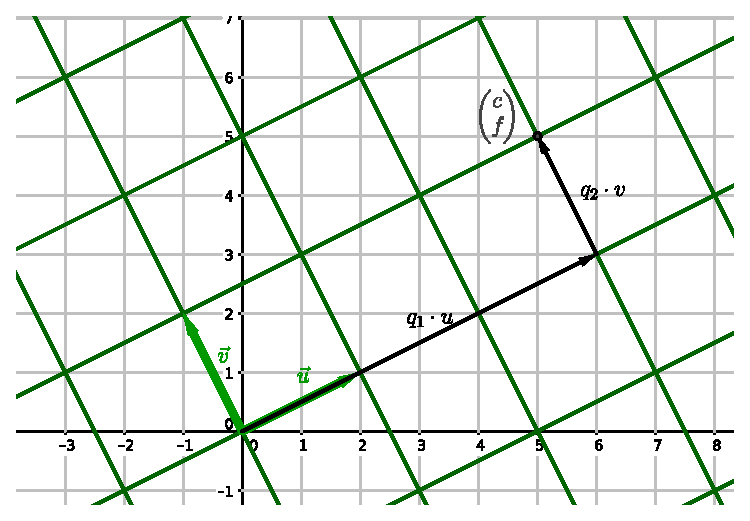
\includegraphics[scale=0.7]{cambio_base.eps}
\end{center}
Possiamo quindi ottenere le coordinate $p_1'$ e $p_2'$, corrispondenti di $p_1$ e $p_2$ nel sistema di riferimento determinato dagli autovettori, utilizzando la formula 
\[
\begin{pmatrix}
	p_1 \\
	p_2
\end{pmatrix}=p_1'\vec{u}+p_2'\vec{v}
\]
Con queste coordinate possiamo riscrivere la precedente rappresentazione matriciale del sistema, ma nel nuovo sistema di riferimento
\begin{align*}
M(p_1'\vec{u}+p_2'\vec{v})&=q_1\vec{u}+q_2\vec{v}\\
p_1'M(\vec{u})+p_2'M(\vec{v})&=q_1\vec{u}+q_2\vec{v}
\end{align*}
Dato che $\vec{u}$ e $\vec{v}$ sono autovettori

\[
p_1'\lambda_1\vec{u}+p_2'\lambda_2\vec{v}=q_1\vec{u}+q_2\vec{v}
\]

Dato che le coordinate di un vettore rispetto alle basi del sistema cartesiano sono uniche, l'equazione precedente è equivalente al seguente sistema
\[
\begin{cases*}
	\lambda_1p_1'=q_1 \\
	\lambda_2p_2'=q_2	
\end{cases*}
\]
Risolvendo il sistema troviamo che $p_1'=\frac{q_1}{\lambda_1}$ e $p_2'=\frac{q_2}{\lambda_2}$\\
Possiamo quindi trovare le soluzioni $p_1$ e $p_2$ del sistema iniziale riportando $p_1'$ e $p_2'$ nel sistema di riferimento originale.
\[
\begin{pmatrix}
	p_1 \\
	p_2
\end{pmatrix}
=
p_1\vec{u}+p_2\vec{v}
\]


\end{document}\grid
